
\documentclass[aspectratio=169]{beamer}
\usepackage{graphicx}  % Required for image inclusion
\usepackage{adjustbox}
\usepackage{caption} 
% Oxford Maths theming
\usetheme{oxfordmaths}

% Set author etc info
\title[Fiedlers Theory of Spectral Graph Partitioning] %short version of title for slide footer
{Fiedlers Theory of Spectral Graph Partitioning} %full title for titlepage
\author{Ayushman Anupam (MDS202411) \\ Biswajit Kala (MDS202412) \\ Boda Sowmya (MDS202413)}
\institute{Data Science\\Chennai Mathematical Institute}
\date[18 May 2024]  %short date for slide footer



%% Now for the actual slides %%
\begin{document}

\begin{frame}[plain]
  \titlepage
\end{frame}
\begin{frame}{Problem Statement}

\begin{columns}

    % Left column with text
    \begin{column}{0.6\textwidth}
        \textbf{Motivation:} Large graphical data structures can be difficult to store and process. \\
        In case of tabular data, we can easily split it into multiple smaller tables. But what if the data is graphical and interconnected? 

        \vspace{0.3cm}
        \textbf{Challenge:}  
        \begin{itemize}
            \item How do we efficiently store, manage, and analyze large graph data?
        \end{itemize}
    \end{column}

    % Right column with image
    \begin{column}{0.4\textwidth}
        \begin{figure}
            \centering
            
\includegraphics[width=\textwidth]{Maths-Beamer-Overleaf/images/image07.jpg}
            \caption*{\small Large Graph}
        \end{figure}
    \end{column}

\end{columns}

\end{frame}

\begin{frame}{Solution Overview}

\begin{columns}

    % Left column with text
    \begin{column}{0.6\textwidth}
        \textbf{Solution Idea:}
        \begin{itemize}
            \item Partition the large graph into smaller, manageable subgraphs.
            \item Store these subgraphs and record the relationships between them.
        \end{itemize}

        \vspace{0.3cm}
        For this, we use a graph partitioning method called \textbf{Fiedler's Spectral Graph Partitioning.}

        \vspace{0.3cm}
        \textbf{In this presentation, we will discuss:}
        \begin{itemize}
            \item How it works
            \item Why it works (correctness)
            \item Implementation examples
        \end{itemize}
    \end{column}

    % Right column with image
    \begin{column}{0.4\textwidth}
        \begin{figure}
            \centering
            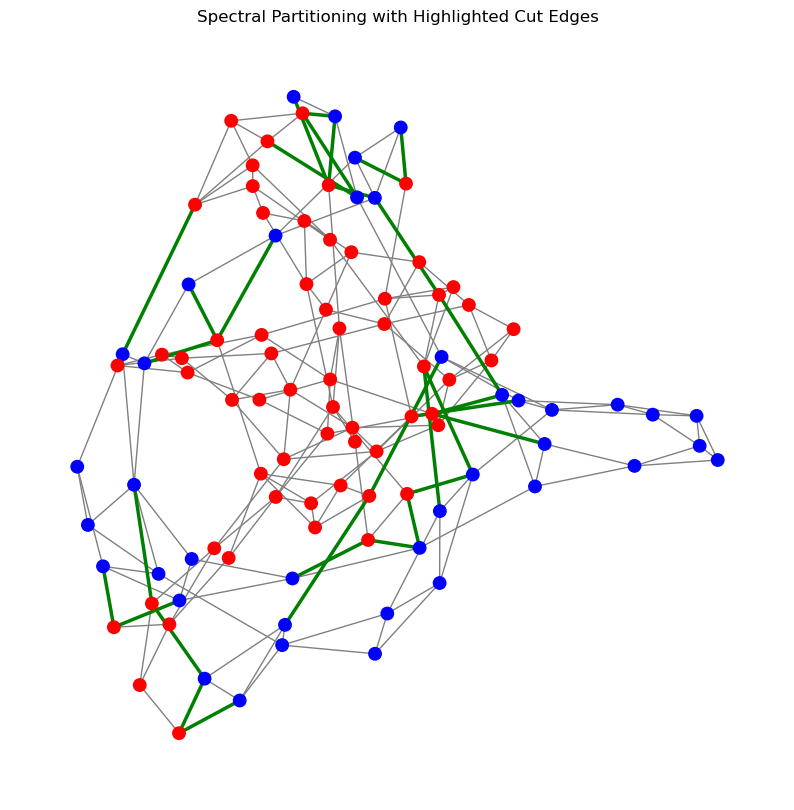
\includegraphics[width=\textwidth]{Maths-Beamer-Overleaf/images/image08.png}
            \caption*{\small Partitioned Graph Example}
        \end{figure}
    \end{column}

\end{columns}

\end{frame}






\begin{frame}{Abstract}
\begin{itemize}
    \item Solution focuses on dividing a connected graph \( G \) into two subgraphs to minimize the number of edges between them.
    
    \item It explores \textbf{spectral graph partitioning}, a method proposed by Fiedler using the Laplacian matrix and its eigenvectors. Vertices of \( G \) are split using one of the eigenvectors of the Laplacian matrix.
    
    \item Presentation conatins Fiedler’s theorem claiming that subgraphs produced by this method are connected.
    
    \item Demonstrates the method on small example graphs to show how effectively it partitions them.
\end{itemize}
\end{frame}


\begin{frame}{Introduction}

Spectral graph partitioning partitions a graph into subgraphs satisfying the following properties:
\begin{itemize}  
    \item The partition divides the graph into two connected subgraphs.
    \item The number of vertices in each of the two subgraphs is nearly equal.
    \item The method minimizes the number of edges connecting the two subgraphs (i.e., the number of edges cut during partition).
\end{itemize}

Key points we are going to see:
\begin{itemize}
    \item Partition is done using the \textbf{eigenvalues and eigenvectors} of the Laplacian matrix associated with the graph.
    \item The spectrum (eigenvalues) of a matrix determines the structure and properties of the partition.
    \item The paper presents Fiedler's technique to perform spectral graph partitioning.
    \item It restates the theorem that the subgraphs generated via spectral partitioning are connected.
\end{itemize}
\end{frame}


\begin{frame}{Overview of Presentation}
In this presentation, we aim to understand how spectral graph partitioning works by exploring the following key points:
\begin{itemize}
    \item Graph Theory and Matrices associated to it.
    \item The \textbf{existence} of a suitable partition in any connected graph.
    \item A proof of how this method \textbf{minimizes the loss of edges (information)} between the subgraphs.
    \item The idea of a \textbf{partition line} (using eigenvectors) and why it effectively separates the graph.
    \item Demonstrating the \textbf{connectedness of the resulting subgraphs} after partitioning. 
    \item Some Examples
    \item Application, limitations and future work
\end{itemize}
\end{frame}



\begin{frame}{Introduction to Graph Theory}


\begin{itemize}
    \item A \textbf{graph} \( G = (V, E) \) is simple, undirected, and has Vertices \( V \), Edges \( E \) connecting vertex pairs \( (u,v) \in E \)
    \item Vertices are labeled with unique integers \( 1, 2, \ldots, |V| \).
    \item The \textbf{degree} of a vertex \( v \), denoted \( d(v) \), is the number of edges incident on \( v \).
\end{itemize}

\subsection*{Graph Matrices}

\begin{itemize}
    \item \textbf{Adjacency Matrix} \( A(G) = (a_{i,j}) \):
    \[
    a_{i,j} = 
    \begin{cases}
        1 & \text{if } (i, j) \in E \\
        0 & \text{otherwise}
    \end{cases}
    \]

    \item \textbf{Degree Matrix} \( D(G) = (d_{i,j}) \):
    \[
    d_{i,j} = 
    \begin{cases}
        d(i) & \text{if } i = j \\
        0 & \text{otherwise}
    \end{cases}
    \]

    \item \textbf{Laplacian Matrix}:
    \(
    L(G) = D(G) - A(G)
    \)
\end{itemize}
\end{frame}

\begin{frame}{Examples}
\vspace{4mm}

% Headings row
\begin{columns}

\begin{column}{0.25\textwidth}
\centering \textbf{\(Graph - G\)}
\end{column}

\begin{column}{0.25\textwidth}
\centering \textbf{Degree Matrix}\\ \textbf{\(D(G)\)}
\end{column}

\begin{column}{0.25\textwidth}
\centering
\textbf{Adjacency Matrix}\\ \textbf{\(A(G)\)}
\end{column}

\begin{column}{0.25\textwidth}
\centering
\textbf{Laplacian Matrix}\\ \textbf{\(L(G) = D(G) - A(G)\)}
\end{column}

\end{columns}

\vspace{3mm}

% First example row
\begin{columns}

\begin{column}{0.25\textwidth}
\centering
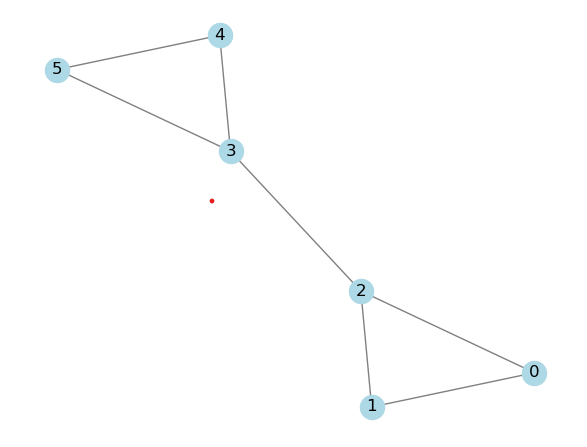
\includegraphics[width=.8\linewidth]{Maths-Beamer-Overleaf/images/image00.png}
\end{column}

\begin{column}{0.25\textwidth}
\centering
\scriptsize
\adjustbox{max width=\linewidth}{
\[
\begin{bmatrix}
2 & 0 & 0 & 0 & 0 & 0 \\
0 & 2 & 0 & 0 & 0 & 0 \\
0 & 0 & 3 & 0 & 0 & 0 \\
0 & 0 & 0 & 3 & 0 & 0 \\
0 & 0 & 0 & 0 & 2 & 0 \\
0 & 0 & 0 & 0 & 0 & 2 \\
\end{bmatrix}
\]}
\end{column}

\begin{column}{0.25\textwidth}
\centering
\scriptsize
\adjustbox{max width=\linewidth}{
\[
\begin{bmatrix}
0 & 1 & 1 & 0 & 0 & 0 \\
1 & 0 & 1 & 0 & 0 & 0 \\
1 & 1 & 0 & 1 & 0 & 0 \\
0 & 0 & 1 & 0 & 1 & 1 \\
0 & 0 & 0 & 1 & 0 & 1 \\
0 & 0 & 0 & 1 & 1 & 0 \\
\end{bmatrix}
\]}
\end{column}

\begin{column}{0.25\textwidth}
\centering
\scriptsize
\adjustbox{max width=\linewidth}{
\[
\begin{bmatrix}
2 & -1 & -1 & 0 & 0 & 0 \\
-1 & 2 & -1  & 0 & 0 & 0 \\
-1 & -1 & 3  & -1  & 0 & 0 \\
0  & 0 & -1 & 3  & -1  & -1 \\
0  & 0  & 0 & -1 & 2  & -1 \\
0  & 0  & 0  & -1 & -1 & 2 \\
\end{bmatrix}
\]}
\end{column}

\end{columns}

\vspace{2mm}

% Second example row
\begin{columns}

\begin{column}{0.25\textwidth}
\centering
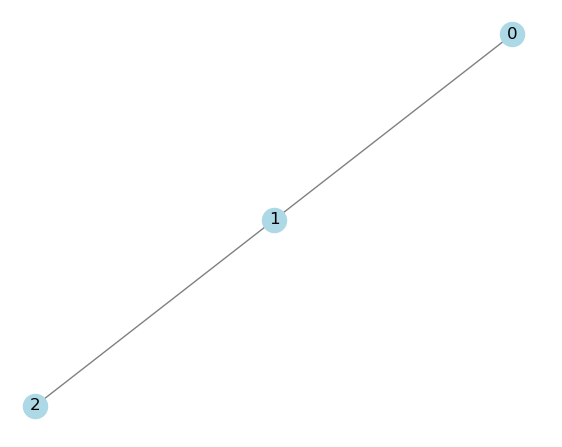
\includegraphics[width=.7\linewidth]{Maths-Beamer-Overleaf/images/image03.png}
\end{column}

\begin{column}{0.25\textwidth}
\centering
\scriptsize
\adjustbox{max width=\linewidth}{
\[
\begin{bmatrix}
1 & 0 & 0 \\
0 & 2 & 0 \\
0 & 0 & 1 \\
\end{bmatrix}
\]}
\end{column}

\begin{column}{0.25\textwidth}
\centering
\scriptsize
\adjustbox{max width=\linewidth}{
\[
\begin{bmatrix}
0 & 1 & 0 \\
1 & 0 & 1 \\
0 & 1 & 0 \\
\end{bmatrix}
\]}
\end{column}

\begin{column}{0.25\textwidth}
\centering
\scriptsize
\adjustbox{max width=\linewidth}{
\[
\begin{bmatrix}
1 & -1 & 0 \\
-1 & 2 & -1 \\
0  & -1 & 1 \\
\end{bmatrix}
\]}
\end{column}

\end{columns}
\end{frame}




\begin{frame}{Eigenvalues and Eigenvectors of L(G)}

\begin{itemize}
    \item For \( A \in \mathbb{R}^{n \times n} \) and a vector \( \mathbf{x} \in \mathbb{R}^n \), if \( A \mathbf{x} = \lambda \mathbf{x} \), then:
    \begin{itemize}
        \item \( \mathbf{x} \) is an \textbf{eigenvector}
        \item \( \lambda \) is the corresponding \textbf{eigenvalue}
    \end{itemize}

    \item An \( n \times n \) matrix has at most \( n \) eigenvalue-eigenvector pairs.

    \item Repeated eigenvalues can occur, but with possibly different eigenvectors.

    \item Eigenvalues are solutions to:
    \[
    \det(A - \lambda I_n) = 0
    \]

    \item Eigenvectors are found by solving:
    \[
    (A - \lambda I_n) \mathbf{x} = \mathbf{0}
    \]
    \item \textbf{Note:} \( \lambda_{1} \) (Smallest eigenvalue) of \( L(G) \) is always 0 and it is positive semi definite.
\end{itemize}
\end{frame}
\begin{frame}{Method of Spectral Graph Partitioning}

Fiedler’s theory of spectral graph partitioning is based upon a very simple idea. For a graph \( G = (V, E) \) which is to be partitioned:

\begin{itemize}
    \item The Laplacian matrix \( L(G) \) is formed.
    \item The eigenvalue-eigenvector pairs of \( L(G) \) are calculated.
    \item Label the eigenvalues so that \( \lambda_1 \leq \lambda_2 \leq \cdots \leq \lambda_n \).
    \item The eigenvector \( \mathbf{x}_2 \), which corresponds to \( \lambda_2 \) (the second-smallest eigenvalue), is known as the \textit{Fiedler vector}, and is used to partition the vertices.
\end{itemize}

Let \( n = |V| \). Recall:

\begin{itemize}
    \item Each of the \( n \) vertices of \( G \) is assigned a unique label from the set \( \{1, 2, \ldots, n\} \).
    \item \( L(G) \in \mathbb{R}^{n \times n} \), and \( \mathbf{x}_2 \in \mathbb{R}^n \).
    \item Therefore, each vertex corresponds to a single entry of \( \mathbf{x}_2 \); that is, vertex \( i \) corresponds to entry \( x_i \) in \( \mathbf{x}_2 \).
\end{itemize}
\end{frame}
\begin{frame}
    

To form the partition:

\begin{itemize}
    \item Create two graphs \( G_1 \) and \( G_2 \).
    \item For each vertex \( i \in G \), if \( x_i < 0 \), assign vertex \( i \) to \( G_1 \); otherwise, assign it to \( G_2 \).
\end{itemize}
\vspace{2mm}
\textbf{Examples 01}
% --- Insert Image Here ---

\noindent
\begin{minipage}[c]{0.4\textwidth}
    \centering
    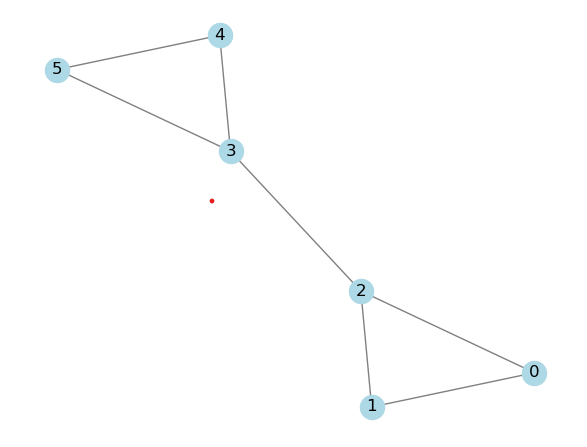
\includegraphics[width=0.9\textwidth]{Maths-Beamer-Overleaf/images/image00.png}
    \captionof{figure}{\textbf{Input Graph}}
\end{minipage}%
\begin{minipage}[c]{0.2\textwidth}
    \centering
    % \textbf{Fiedler's Vector:}
    \[
    \begin{bmatrix}
    0.4647 \\
    0.4647 \\
    0.2610 \\
    -0.2610 \\
    -0.4647 \\
    -0.4647 \\
    \end{bmatrix}
    \]
    \textbf{Fiedler's Vector}
\end{minipage}%
\hfill
\begin{minipage}[c]{0.3\textwidth}
    \centering
    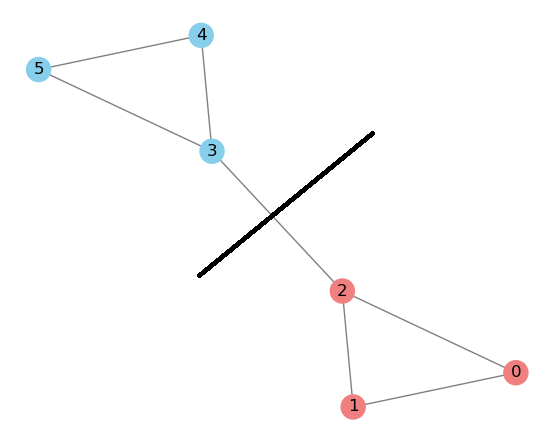
\includegraphics[width=0.9\textwidth]{Maths-Beamer-Overleaf/images/image01.png}
    \captionof{figure}{\textbf{Partitioned Subgraph}}
\end{minipage}
\end{frame}


\begin{frame}
\textbf{Examples 02}\\
\noindent
\begin{minipage}[c]{0.4\textwidth}
    \centering
    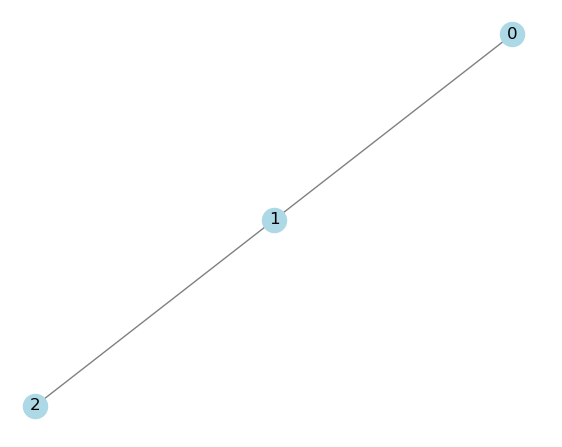
\includegraphics[width=0.9\textwidth]{Maths-Beamer-Overleaf/images/image03.png}
    \captionof{figure}{\textbf{Input Graph}}
\end{minipage}%
\begin{minipage}[c]{0.2\textwidth}
    \centering
    % \textbf{Fiedler's Vector:}
    \[
    \begin{bmatrix}
    -0.7071 \\
    0.0001 \\
    0.7071 \\
    \end{bmatrix}
    \]
    \textbf{Fiedler's Vector}
\end{minipage}%
\hfill
\begin{minipage}[c]{0.4\textwidth}
    \centering
    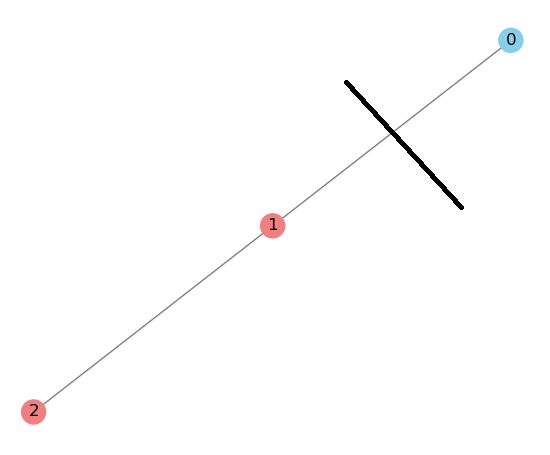
\includegraphics[width=0.9\textwidth]{Maths-Beamer-Overleaf/images/image04.png}
    \captionof{figure}{\textbf{Partitioned Subgraph}}
\end{minipage}

This defines a partition of \( G \) into two sets. However, it is not evident that this partition minimizes the number of edges between \( G_1 \) and \( G_2 \), or even that the two subgraphs are connected.
\end{frame}
%%%%%%%%%%%%%%%%%%%%%%%%%%%%%%%%%%%%%%%%%%%%%%%%%%%%%%%%%%%%%%%%%%%%%%%%%%
\begin{frame}{Why Second-Smallest Eigenvector — Standing Wave Analogy}

To explain why Fiedler's partition works, we use the example of a vibrating string.

\begin{figure}
    \centering
    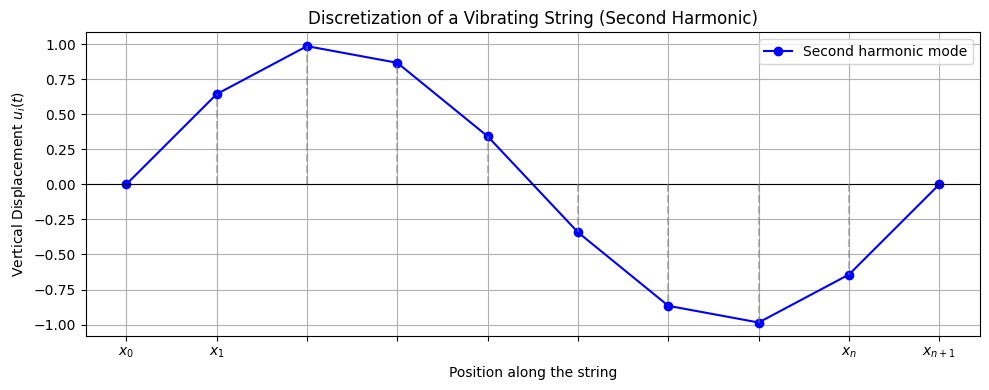
\includegraphics[width=0.7\textwidth]{Maths-Beamer-Overleaf/images/image02.jpg}
    \caption{Illustration of a vibrating string}
\end{figure}

Consider a string of length \( L \), discretized into \( n+1 \) equal segments, resulting in \( n \) interior points and two fixed boundary points at \( x_0 = 0 \) and \( x_{n+1} = L \). Here, each \( x_i \) can be viewed as a vertex in a graph.
\end{frame}

\begin{frame}

\textbf{Note:} The above is a \textit{chain graph}, where each intermediate vertex has degree 2, and the two end vertices have degree 1. It represents a simple, linear sequence of connected vertices.

\vspace{0.3cm}

\textbf{Segment length:}
\[
h = \frac{L}{n+1}, \quad x_i = i \cdot h, \quad i = 0, 1, \dots, n+1.
\]

As \( n \to \infty \), \( h \to 0 \) i.e, the discrete chain graph approaches a continuous string. \\
This allows us to model the entire string as a chain graph. Relating this to the \textit{standing wave theory}, we have:

\begin{itemize}
    \item Vertical displacement at position \( x_i \): \( u_i(t) \).
    \item Fixed boundary conditions: \( u_0(t) = 0, \quad u_{n+1}(t) = 0 \).
    \item Displacement vector for interior points:
    \[
    \mathbf{u}(t) = \begin{bmatrix} u_1(t), u_2(t), \vdots, u_n(t) \end{bmatrix}^t.
    \]
\end{itemize}

\end{frame}

\begin{frame}
    
        \textbf{Note: Continuous wave equation } \(
        \frac{\partial^2 u}{\partial t^2} = c^2 \frac{\partial^2 u}{\partial x^2}.  \)
    \begin{itemize}
        \item In our case, Discrete second spatial derivative using central finite difference gives:
        \[
        \frac{\partial^2 u_i}{\partial x^2} \approx \frac{u_{i-1} - 2u_i + u_{i+1}}{h^2}.
        \]
        \\
         Writing it in matrix form foe all \(x_i\) gives matrix \( \mathbf{D} \):
        \[
        \mathbf{D} = \begin{bmatrix}
            -2 & 1 & 0 & \cdots & 0 \\
            1 & -2 & 1 & \cdots & 0 \\
            0 & 1 & -2 & \cdots & 0 \\
            \vdots & \vdots & \ddots & \ddots & \vdots \\
            0 & 0 & \cdots & 1 & -2
        \end{bmatrix}.
        \]
        \item which exactly looks like the Laplacian matrix of the chain graph.
    \end{itemize}
\end{frame}

\begin{frame}

\begin{itemize}
    \item Substituting into the discrete wave equation:
    \[
    \frac{d^2 \mathbf{u}}{dx^2} \approx \frac{1}{h^2} \mathbf{D} \mathbf{u}
    \]
    \[
    \implies \frac{d^2 \mathbf{u}}{dt^2} = \frac{c^2}{h^2} \mathbf{D} \mathbf{u}
    \]

    \item From the equation of a standing wave:
    \[
    \frac{d^2 \mathbf{u}}{dt^2} = -\omega^2 \mathbf{u}
    \]

    \item Comparing both, we arrive at the eigenvalue problem:
    \[
    \mathbf{D} \mathbf{u} = -\frac{\omega^2 h^2}{c^2} \mathbf{u}
    \]

    \item \textbf{Note:} which is exactly the eigenvalue equation, with eigenvalue:
    \[
    \lambda = \frac{-\omega^2 h^2}{c^2}
    \]
\end{itemize}

\end{frame}


\begin{frame}

\textbf{Note:} The eigenvalues of \( \mathbf{D} \) are given by:
\[
\lambda_k = 2\left(1 - \cos\left(\frac{k \pi}{n+1}\right)\right), \quad k = 1, 2, \dots, n
\]
where the eigenvalues are ordered as:
\[
\lambda_1 < \lambda_2 < \cdots < \lambda_n
\]

\begin{itemize}
    \item The second smallest eigenvalue \( \lambda_2 \) is:
    \[
    \lambda_2 = 2\left(1 - \cos\left(\frac{2 \pi}{n+1}\right)\right)
    \]
    
    \item The corresponding natural frequency associated with \( \lambda_2 \) is:
    \[
    \omega = 2 \pi f = \sqrt{\frac{c^2 \lambda_2}{h^2}}
    \]
\end{itemize}

\end{frame}



\begin{frame}

\begin{itemize}
    \item The corresponding frequency \( f \) is equal to the second harmonic \( \frac{c}{L} \) of the standing wave. This mode divides the particles of the string into two groups — half with upward acceleration and half with downward acceleration. 
    Similarly, the chain graph is partitioned into two parts with nearly equal numbers of vertices.
    
    \item From our earlier discussion, we observed that the second eigenvector of the Laplacian matrix \( L(G) \) partitions a chain graph into two nearly equal halves.

    \item For more complex graphs beyond simple chains, the same intuition holds. It is particularly intuitive in planar graphs, which can be visualized like a trampoline — where the second mode of vibration similarly divides the graph (or trampoline) into two balanced regions.
\end{itemize}

\end{frame}

















































%%%%%%%%%%%%%%%%%%%%%%%%%%%%%%%%%%%%%%%%%%%%%%%%%%%%%%%%%%%%%%%%%%%%%%%%%%%5

\begin{frame}{Correctness of Partition - Mathematical View}
    \textbf{Note:}The smallest eigenvalue of \( L(G) \) is \( \lambda_1 = 0 \), and eigenvector associated with \( \lambda_1 \) is \( \mathbf{v}_{\lambda_1} = [1, 1, \dots, 1]_{n \times 1} \).

    
    Since smallest eigenvalue of \( L(G) \) is \( 0 \), we focus on the second smallest eigenvalue \( \lambda_2 \).

    \[
    \lambda_2 = \min_{\mathbf{x} \perp \mathbf{1}} \frac{\mathbf{x}^T L \mathbf{x}}{\mathbf{x}^T \mathbf{x}}
    \]

    \[
    = \min \sum_{i=1}^n \sum_{j=1}^n (D_{ij} - A_{ij}) x_i x_j 
    = \sum_{i} D_{ii} x_i^2 - 2 \sum_{(i,j) \in E} x_i x_j
    \]

    \[
    = \min \sum_{(i,j) \in E} \left( x_i^2 + x_j^2 - 2 x_i x_j \right)
    = \min \sum_{(i,j) \in E} (x_i - x_j)^2
    \]

    \textbf{Note:} Here, each \( x_i \) is associated with a node.
\end{frame}

\begin{frame}
    Since \( \mathbf{v}_{\lambda_1} \) and \( \mathbf{x} = [x_1, x_2, \dots, x_n]^T \) are orthogonal eigenvectors:

    \[
    \mathbf{v}_{\lambda_1}^T \mathbf{x} = \sum_{i=1}^n x_i = 0
    \]

    \vspace{0.3cm}

    \textbf{Therefore:}
    \begin{itemize}
        \item Some labels \( x_i \) are negative, and some are positive.
        \item This naturally induces a partition of the graph into two sets:
        \begin{itemize}
            \item Nodes with \( x_i < 0 \)
            \item Nodes with \( x_i \geq 0 \)
        \end{itemize}
        \item Hence, a \textbf{partition exists} based on the sign of the entries in the eigenvector corresponding to \( \lambda_2 \).\\
        \hfill \(\blacksquare\)
    \end{itemize}
\end{frame}

\begin{frame}
    So, the problem statement becomes:

    \[
    \lambda_2 = \min_{\text{all labelings of nodes s.t. } \sum_i x_i = 0} \sum_{(i,j) \in E} (x_i - x_j)^2
    \]

    \textbf{Note:} The above summation is minimized when \( x_i \) and \( x_j \) have the same sign for each \( (i, j) \in E \). \\
    If they have different signs, the term \( (x_i - x_j)^2 \) increases, raising the overall summation.

    \vspace{0.3cm}

    This minimization ensures that the number of edges connecting nodes with different signs is as small as possible. 
    In the context of graph partitioning:
    \begin{itemize}
        \item It minimizes the number of edges that are cut during the partition.
        \item Encourages connected nodes to remain within the same partition.
    \end{itemize}

     \vspace{0.3cm}
\end{frame}






\begin{frame}{Balanced Partitioning Insight}

\textbf{Moreover:} 
To minimize the above summation, we aim to reduce the total number of terms in the summation. Ideally, this is achieved when the number of vertices in both subgraphs is approximately equal.

\vspace{0.3cm}

\textbf{Note:} 
This condition does not always hold — it is a weak assumption. However, in most cases, balancing the number of vertices helps minimize the total number of possible \( (x_i, x_j) \) pairs across partitions, which effectively reduces the total cut value.

\vspace{0.3cm}

\textbf{Hence,} this method of partitioning ensures:
\begin{itemize}
    \item The number of vertices in both partitions remains balanced.
    \item The number of edges cut between partitions is minimized.
\end{itemize}

\hfill \(\blacksquare\)

\end{frame}








%%%%%%%%%%%%%%%%%%%%%%%%%%%%%%%%%%%%%%%%%%%%%%%%%%%%%%%%%%%%%%%%%%
\begin{frame}
\begin{figure}[H]
    \centering
    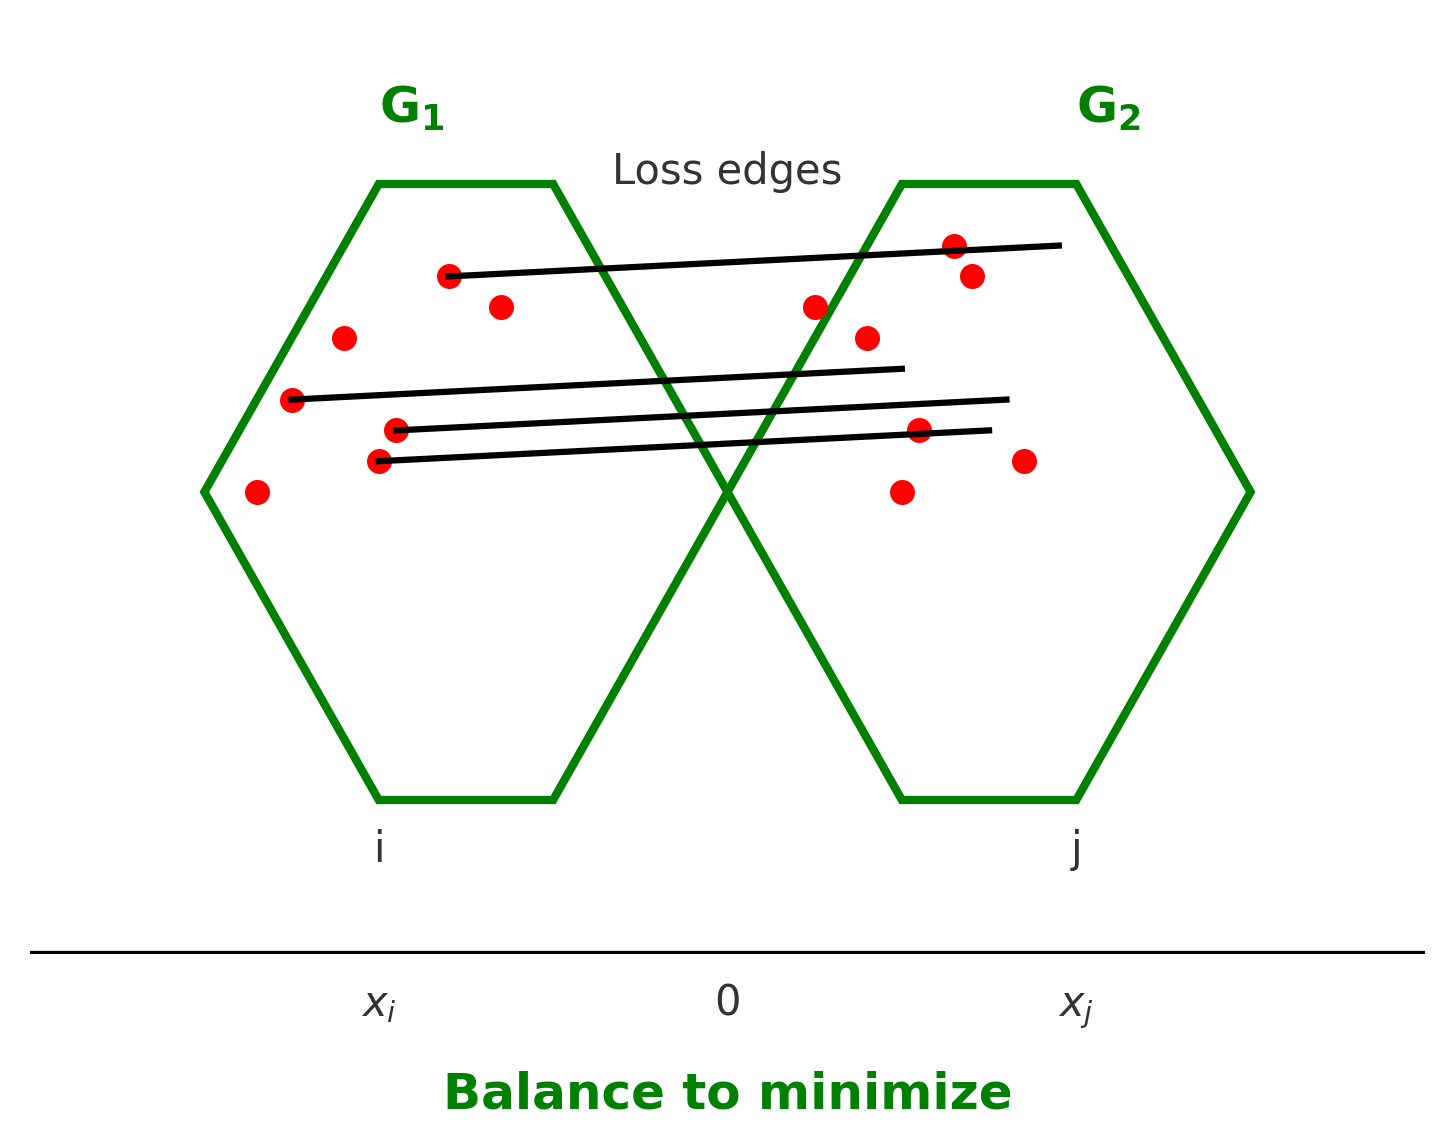
\includegraphics[width=0.7\textwidth]{Maths-Beamer-Overleaf/images/partition_graph.png}
    \label{fig:partition_graph}
\end{figure}
\end{frame}

%%%%%%%%%%%%%%%%%%%%%%%%%%%%%%%%%%%%%%%%%%%%%%%%%%%%%%%%%%%%%%%%%

\begin{frame}{what we did and Next Steps}
    \textbf{So far, we have shown:}
    \begin{itemize}
        \item A valid partition exists.
        \item The partition minimizes the number of lost (cut) edges.
        \item It ensures that the number of vertices in each subgraph is balanced.
    \end{itemize}
    
    \vspace{0.5cm}
    \textbf{What remains is to prove:} \\
    That the two subgraphs obtained from the partition are \textbf{connected}.

    \vspace{0.5cm}
    One of \textbf{Fiedler's key contributions} was proving that the two subgraphs formed through spectral partitioning are always connected. \\
    
    Before presenting his proof, we will follow \textbf{Demmel's approach}, introducing some essential definitions and lemmas to build up the argument.
\end{frame}


\begin{frame}{\textbf{Some Linear Algebra Definition }}
 \textbf{\large Definition 1: Non-negative Matrix} 
  A matrix $A$ is said to be \textit{non-negative} if all of its elements are greater than or equal to zero, i.e.,
  \[    a_{ij} \geq 0 \quad \text{for all } i, j.  \]
  
  
  
  \textbf{\large Definition 2: Spectral Radius}  
  The \textit{spectral radius} of a square matrix $A$ is the largest absolute value among its eigenvalues. It is denoted by:
  \[    \rho(A) = \max_i |\lambda_i|,  \]
  where $\lambda_1, \lambda_2, \ldots, \lambda_n$ are the eigenvalues of the matrix $A$.  
\end{frame}


\begin{frame}
\textbf{\large Definition 3: Positive Definite Matrix}  
  A square matrix $A$ is called \textit{positive definite} if:
  \[
    x^T A x > 0 \quad \text{for all non-zero vectors } x.
  \]

  \vspace{1em}

  \textbf{\large Remark 4: Symmetric and Positive-Definite Matrices}  
  The matrix $A$ is symmetric and positive definite if and only if every eigenvalue of $A$ is positive. 
  
  In addition, $A$ is symmetric and positive semi-definite if and only if every eigenvalue of $A$ is nonnegative. 
\end{frame}

\begin{frame}{\textbf{Lemmas and Theorem from Linear Algebra}}
    \textbf{Lemma 5.}  
If \( A \) is an \( n \times n \) symmetric matrix with eigenvalues \( \lambda_1 \leq \lambda_2 \leq \cdots \leq \lambda_n \), then
\[
\lambda_1 = \min_{v \neq 0} \frac{v^T A v}{v^T v}, \quad \lambda_n = \max_{v \neq 0} \frac{v^T A v}{v^T v}.
\]
That is, \( \lambda_1 \) and \( \lambda_n \) are the minimum and maximum values of the expression \( \frac{v^T A v}{v^T v} \) taken over all nonzero vectors \( v \in \mathbb{R}^n \).

\textbf{Proof.}  
Let \( v \in \mathbb{R}^n \) be any non-zero vector. Define the Rayleigh quotient:
\[
R(v) = \frac{v^T A v}{v^T v}.
\]
Let \( y = \frac{v}{\|v\|} \), so \( \|y\| = 1 \), and thus \( R(v) = y^T A y \).
\end{frame}

\begin{frame}
    

Since \( A \) is symmetric, it is orthogonally diagonalizable. That is,
\(
A = Q \Lambda Q^T,
\)
where \( Q \) is an orthogonal matrix and \( \Lambda = \text{diag}(\lambda_n \lambda_(n-1), \ldots, \lambda_1) \).

Then,
\[
y^T A y = y^T Q \Lambda Q^T y = (Q^T y)^T \Lambda (Q^T y).
\]
Let \( z = Q^T y \), so \( \|z\| = \|y\| = 1 \). Then,
\[
\frac{v^T A v}{v^T v} = z^T \Lambda z = \sum_{i=1}^n \lambda_{n - i + 1} z_i^2 = z_1^2 \lambda_n + z_2^2 \lambda_{n-1} + \cdots + z_n^2 \lambda_1,
\]


Since \( \sum_{i=1}^n z_i^2 = 1 \), this is a convex combination of the eigenvalues \( \lambda_i \). Therefore,
\[
\lambda_1 \leq R(v) \leq \lambda_n.
\]

Hence,
\[
\min_{v \neq 0} \frac{v^T A v}{v^T v} = \lambda_1, \quad \max_{v \neq 0} \frac{v^T A v}{v^T v} = \lambda_n.
\]
\hfill \(\blacksquare\)

\end{frame}

\begin{frame}{\textbf{Theorem 6 - Cauchy Interlacing Theorem}}
\textbf{Cauchy Interlacing Theorem}  
Let \( A \in \mathbb{R}^{n \times n} \) be a symmetric matrix with eigenvalues ordered as
\[
\lambda_1 \leq \lambda_2 \leq \cdots \leq \lambda_n.
\]

Let \( A(i{:}j, i{:}j) \) denote the principal submatrix of \( A \), formed by taking rows and columns \( i \) through \( j \), so that \( A(i{:}j, i{:}j) \in \mathbb{R}^{(j-i+1) \times (j-i+1)} \). 

Let the eigenvalues of \( A(i{:}j, i{:}j) \) be
\[
\chi_1 \leq \chi_2 \leq \cdots \leq \chi_{j - i + 1}.
\]

Then for any \( k \leq j - i + 1 \), the matrix \( A \) has at least \( k \) eigenvalues that are less than or equal to \( \chi_k \); that is,
\[
| \{ \lambda_\ell \mid \lambda_\ell \leq \chi_k \}| \geq k.
\]
\end{frame}

\begin{frame}{ Cauchy Interlacing theorem simplified}
    \begin{itemize}
        \item Consider any symmetric matrix \( A \) of size \( n \times n \), with eigenvalues ordered as:
        \[
        \lambda_n \geq \lambda_{n-1} \geq \cdots \geq \lambda_1
        \]
        \item Let \( A_m \) be a submatrix of \( A \) of size \( m \times m \) (with \( n > m \)) having eigenvalues:
        \[
        \chi_m \geq \chi_{m-1} \geq \cdots \geq \chi_1
        \]
        \item Then for any \( k \in \{1, 2, \dots, m\} \), we must have at least \( k \) eigenvalues of \( A \) less than or equal to the \( k \)-th largest eigenvalue of \( A_m \), that is:
        \[
        \left| \left\{ \lambda_\ell \mid \lambda_\ell \leq \chi_k \right\} \right| \geq k
        \]
    \end{itemize}
\end{frame}

\begin{frame}{Example: Cauchy Interlacing Theorem}

Consider symmetric matrix \( A \) and its submatrix \( A_2 \):
\[
A = \begin{bmatrix}
4 & 1 & 0 & 0 \\
1 & 3 & 0 & 0 \\
0 & 0 & 2 & 0 \\
0 & 0 & 0 & 1 
\end{bmatrix}, \quad
A_2 = \begin{bmatrix}
4 & 1 \\
1 & 3
\end{bmatrix}
\]

Eigenvalues:
\begin{itemize}
    \item For \( A \): \( \lambda = \{4.618, 3.382, 2, 1\} \)
    \item For \( A_2 \): \( \chi = \{4.618, 2.382\} \)
\end{itemize}

\textbf{Check Interlacing:}
\begin{itemize}
    \item k = 2: \(\chi_2 = 4.618  \geq  \lambda_2 = 3.382 \geq  \lambda_1 = 1 \)
    \item k = 1:  \(\chi_1 = 2.382  \geq  \lambda_1 = 1 \)
\end{itemize}
\end{frame}


\begin{frame}{\textbf{Theorem 7}}
\textbf{
Let \( A \) be a \( n \times n \) matrix and let \( X \) be any \( n \times n \) non-singular matrix. Then \( X^T A X \) is symmetric positive-definite if and only if \( A \) is symmetric positive-definite.}
\\
\textbf{Proof ( \( \impliedby\) direction):}

Assume \( A \) is symmetric positive definite. Then:
\[
A = A^T \quad \text{and} \quad \lambda_{\min}(A) > 0
\]
We analyze \( X^T A X \):

\textbf{1. Symmetry:  }
   \[
   (X^T A X)^T = X^T A^T X = X^T A X \quad \text{(since \( A = A^T \))}
   \]
   Therefore, \( X^T A X \) is symmetric.
\end{frame}
\begin{frame}
    

\textbf{2. Positive definiteness:}  
   Consider the Rayleigh quotient for \( X^T A X \):
   \[
   \lambda_{\min}(X^T A X) = \min_{v \neq 0} \frac{v^T X^T A X v}{v^T v}
   \]
   Multiply and divide by \( v^T X^T X v \) (valid for all \( v \neq 0 \)):
   \[
   = \min_{v \neq 0} \left( \frac{v^T X^T A X v}{v^T X^T X v} \cdot \frac{v^T X^T X v}{v^T v} \right)
   \]
   Let \( y = Xv \). Then:
   \[
   \frac{v^T X^T A X v}{v^T X^T X v} = \frac{y^T A y}{y^T y} \ge \lambda_{\min}(A)
   \]
   Also:
   \[
   \frac{v^T X^T X v}{v^T v} \ge \lambda_{\min}(X^T X)
   \]

\end{frame}
\begin{frame}
   Hence:
   \[
   \lambda_{\min}(X^T A X) \ge \lambda_{\min}(A) \cdot \lambda_{\min}(X^T X)
   \]

   Since \( X \) is non-singular, \( X^T X \) is also non-singular, so \( \lambda_{\min}(X^T X) > 0 \).  
   Therefore, \( \lambda_{\min}(X^T A X) > 0 \), and so \( X^T A X \) is positive definite.

Thus, \( X^T A X \) is symmetric and positive definite.

    
\vspace{3mm}
\textbf{(\(\implies\) direction)}

Assume \( X^T A X \) is symmetric positive definite. Then:
\[
\lambda_{\min}(X^T A X) > 0
\]

\textbf{1. Symmetry: } 
   \( X^T A X \) is symmetric:
   \[
   (X^T A X)^T = X^T A^T X
   \]
   Since \( X^T A X = X^T A^T X \), we conclude that \( A = A^T \).  
   Therefore, \( A \) is symmetric.
\end{frame}
\begin{frame}
\textbf{2. Positive definiteness:  }
   From earlier, we know:
   \[
   \lambda_{\min}(X^T A X) = \lambda_{\min}(A) \cdot \lambda_{\min}(X^T X)
   \]
   Since \( X \) is nonsingular, \( X^T X \) is also nonsingular, implying \( \lambda_{\min}(X^T X) > 0 \).  
   For the product \( \lambda_{\min}(X^T A X) = \lambda_{\min}(A) \cdot \lambda_{\min}(X^T X) \) to be positive, it follows that \( \lambda_{\min}(A) > 0 \).  
   Therefore, \( A \) is positive definite.



\bigskip

\textbf{Conclusion:}


A is symmetric positive definite \( \iff  X^TAX \)\ is symmetric positive definite (when \( X \) is non singular).
\hfill \(\blacksquare\)
\end{frame}

\begin{frame}{\textbf{Lemma 8}}
\textbf{ Let \( A \) be an \( n \times n \) symmetric matrix. If \( \rho(A) < 1 \), meaning that all eigenvalues of \( A \) is on the interval \( (-1, 1) \), then \( I_n - A \) is nonsingular and:
\[ (I_n - A)^{-1} = \sum_{i=0}^\infty A^i \]}

\textbf{Proof.}

\begin{itemize}

    \item \textbf{Eigenvalues of \( I_n - A \):} \\
    Since \( A \) is symmetric, its eigenvalues are real and lie in \( (-1, 1) \). The identity matrix \( I_n \) has eigenvalues equal to 1. Hence, the eigenvalues of \( I_n - A \) are:
    \[
    \lambda_i(I_n - A) = 1 - \lambda_i(A) \in (0, 2)
    \]
    Therefore, all eigenvalues of \( I_n - A \) are positive, which implies it is nonsingular. 
\end{itemize}
\end{frame}
\begin{frame}
    

\begin{itemize}
   
    \item \textbf{Convergence of the series:} \\
    Since \( A \) is symmetric, we can diagonalize it:
    \(
    A = Q \Lambda Q^T
    \)
    where \( Q \) is orthogonal and \( \Lambda \) is diagonal.
    \\
    Then:
    \(
    A^i = Q \Lambda^i Q^T
    \)
    Since all \( |\lambda_i| < 1 \), \( \Lambda^i \to 0 \) as \( i \to \infty \), and so:
    \( A^i \to 0 \)
    \\
    Thus, the series \( \sum_{i=0}^\infty A^i \) converges.

    \item \textbf{Telescoping sum argument:} \\
    Let \( S_m = \sum_{i=0}^m A^i \). Then:
    \[
    (I_n - A) S_m = (I_n - A)(I_n + A + \dots + A^m) = I_n - A^{m+1}
    \]
    As \( m \to \infty \), \( A^{m+1} \to 0 \), so:
    \[
    (I_n - A) \cdot \sum_{i=0}^\infty A^i = I_n
    \]
    Therefore,
    \(
    (I_n - A)^{-1} = \sum_{i=0}^\infty A^i
    \)
\hfill \(\blacksquare\)
\end{itemize}
\end{frame}

%%%%%%%%%%%%%%%%%%%%%%%%%%%%%%%%%%%%%%%%%%%%%%%%%%%%%%%%%%%%%%%%%%%%%%%%%%

\begin{frame}{Fiedler's Theorem of Spectral Graph Partitioning}


\textbf{Let \( G \) be a connected graph and let \( L(G) \) be its Laplacian matrix. Create the subgraphs \( G_1 \) and \( G_2 \) using Fiedler's method. Then, both \( G_1 \) and \( G_2 \) are connected.}

\textbf{Proof (by contradiction):}
  \begin{itemize}
    \item Assume Without loss of generality \( G_1 \) is composed of two connected components.
    \item Let \( \mathbf{x} \) be the eigenvector corresponding to \( \lambda_2 \), the second-smallest eigenvalue of \( L(G) \).
    \item So both \( L(G) \) and \( \mathbf{x} \) can be written in block form:


  \[
  L(G) = 
  \begin{bmatrix}
  L_{1,1} & O & L_{1,3} \\
  O & L_{2,2} & L_{2,3} \\
  L_{1,3}^T & L_{2,3}^T & L_{3,3}
  \end{bmatrix}
  \quad \text{and} \quad
  \mathbf{x} =
  \begin{bmatrix}
  \mathbf{x}_1 \\
  \mathbf{x}_2 \\
  \mathbf{x}_3
  \end{bmatrix}
  \]

  \item Here, \( \mathbf{x} \) is the Fiedler vector (associated with \( \lambda_2 \)) where \( \mathbf{x}_1 \) and \( \mathbf{x}_2 \) are positive and \( \mathbf{x}_3 \) is negative.
\end{itemize}

\end{frame}




%%%%%%%%%%%%%%%%%%%%%%%%%%%%%%%%%%%%%%%%%%%%%%%%%%%%%%%%%%%%%%%%%%%%%%%%%%%%
\begin{frame}{\textbf{Proof of Fiedler's Theorem (continued)}}

\begin{itemize}
  \item \( O \) denotes a matrix of appropriate size with all entries equal to zero.
  
  \item \textbf{Note: }\( L(G) \) is symmetric. Its Diagonal blocks of are symmetric and  off-diagonal block in position \( (i, j) \) is the transpose of the block in position \( (j, i) \). Also, all off-diagonal blocks are non-positive.


  \item But, Each block \( L_{i,j} \) has same properties, this implies, each Laplacian matrix, corresponds to subgraphs or components of the graph \( G \).

  \item Since, graph is partitioned using the Fiedler vector \( \mathbf{x} \). so, Vertices corresponding to \( \mathbf{x}_1 \) and \( \mathbf{x}_2 \) are grouped into the same subgraph \( G_1 \).

  \item There are no edges between \( \mathbf{x}_1 \) and \( \mathbf{x}_2 \), Since, the entries in \( L(1, 2) \) and \( L(2, 1) \) are 0. which implies: \( G_1 \) is disconnected and its components are represented by Laplacians like \( L_{1,1} \) and others.

\end{itemize}
\end{frame}

%%%%%%%%%%%%%%%%%%%%%%%%%%%%%%%%%%%%%%%%%%%%%%%%%%%%%%%%%%%%%%%%%%%%%%%%

\begin{frame}

\begin{itemize}
  \item Let \( \mathbf{x} \) be an eigenvector of \( L(G) \) with eigenvalue \( \lambda_2 \), so:
  \[
  L(G)\mathbf{x} = \lambda_2 \mathbf{x}.
  \]

  \item Consider the first block \( \mathbf{x}_1 \) of \( \mathbf{x} \). Multiplying out the corresponding block row:
  \[
  L_{1,1}\mathbf{x}_1 + L_{1,3}\mathbf{x}_3 = \lambda_2 \mathbf{x}_1.
  \]

  \item Since all eigenvalues of \( L(G) \) are nonnegative and by the \textbf{Cauchy Interlacing Theorem}, all eigenvalues of \( L_{1,1} \) are also nonnegative.

  \item Let \( \varepsilon > 0 \). Add \( \varepsilon \mathbf{x}_1 \) to both sides of the equation:
  \[
  \varepsilon \mathbf{x}_1 + L_{1,1} \mathbf{x}_1 + L_{1,3} \mathbf{x}_3 = \varepsilon \mathbf{x}_1 + \lambda_2 \mathbf{x}_1.
  \]

  \item This can be written more concisely as:
  \[
  (\varepsilon I + L_{1,1})\mathbf{x}_1 + L_{1,3} \mathbf{x}_3 = (\varepsilon + \lambda_2) \mathbf{x}_1,
  \]
  where \( I \) is the identity matrix of appropriate size.

\end{itemize}
\end{frame}
%%%%%%%%%%%%%%%%%%%%%%%%%%%%%%%%%%%%%%%%%%%%%%%%%%%%%%%%%%%%%%%%%%%%%%%%
\begin{frame}


\begin{itemize}
  \item  \( L_{1,1} \) represents a subgraph of G, so its smallest eigenvalue is \( \ge 0 \). So, by the properties of \( I \) and symmetric matrices, and as discussed in the proof of Lemma 2.8, the eigenvalues of \( \varepsilon I + L_{1,1} \) are all at least \( \varepsilon \), hence:
  \[
  \varepsilon I + L_{1,1} \text{ is positive-definite}.
  \]

  \item Using Demmel’s method, let:
  \[
  \varepsilon I + L_{1,1} = D - N,
  \]
  where:
  \begin{itemize}
    \item \( D \) is diagonal, with each diagonal entry equal to the corresponding diagonal element of \( \varepsilon I + L_{1,1} \),
    \item \( -L \) contains the off-diagonal entries of \( \varepsilon I + L_{1,1} \),
    \item Every diagonal entry of \( -L \) is 0.
  \end{itemize}
\end{itemize}
\end{frame}


%%%%%%%%%%%%%%%%%%%%%%%%%%%%%%%%%%%%%%%%%%%%%%%%%%%%%%%%%%%%%%%%%%%%%%%%%%
\begin{frame}
    

\begin{itemize}

  \item This expression can be further decomposed as:
  \[
  D^{\frac{1}{2}} \left( I - (D^{\frac{1}{2}})^{-1} N (D^{\frac{1}{2}})^{-1} \right) D^{\frac{1}{2}},
  \]
  where \( D^{\frac{1}{2}} \) is the matrix formed by taking the square root of each element of \( D \).

  \item Since \( D \) is diagonal and nonnegative, we have:
  \[
  D^{\frac{1}{2}} D^{\frac{1}{2}} = D.
  \]

  \item Multiply through the decomposition to verify:
  \[
  \varepsilon I + L_{1,1} = D - N.
  \]

  \item Let:
  \[
  M = (D^{\frac{1}{2}})^{-1} N (D^{\frac{1}{2}})^{-1},
  \]
  which implies,
  \[
  \varepsilon I + L_{1,1} = D - N = D^{\frac{1}{2}} (I - M) D^{\frac{1}{2}}.
  \]
\end{itemize}

\end{frame}


%%%%%%%%%%%%%%%%%%%%%%%%%%%%%%%%%%%%%%%%%%%%%%%%%%%%%%%%%%%%%%%%%%%%%%%%
\begin{frame}

\begin{itemize}
  \item Since \( D^{\frac{1}{2}} \) is diagonal, we have:
  \[
  \left( D^{\frac{1}{2}} \right)^T = D^{\frac{1}{2}}.
  \]

  \item From Lemma 2.7 and earlier decomposition:
  \[
  \varepsilon I + L_{1,1} = D^{\frac{1}{2}} (I - M) D^{\frac{1}{2}}
  \Rightarrow (D^{\frac{1}{2}})^T (I - M) D^{\frac{1}{2}} \text{ is positive-definite}.
  \]

  \item Thus, \( I - M \) is also positive-definite.

  \item Using symmetry arguments for eigenvalues:
  \[
  \text{If } \lambda \text{ is an eigenvalue of } M, \text{ then } 1 - \lambda \text{ is an eigenvalue of } I - M.
  \]
    \[
  \implies 1 \ge \lambda_{M}
  \]
\end{itemize}
\end{frame}
%%%%%%%%%%%%%%%%%%%%%%%%%%%%%%%%%%%%%%%%%%%%%%%%%%%%%%%%%%%%%%%%%%%%%%%%
\begin{frame}

\begin{itemize}
  \item From Lemma 2.5   \[
  \lambda_1(M) = \min_{\mathbf{v} \ne 0} \frac{\mathbf{v}^T M \mathbf{v}}{\mathbf{v}^T \mathbf{v}}
  \]

  \[ \implies \lambda_1(M)
  \ge \min_{\mathbf{v} \ne 0} \frac{-|\mathbf{v}|^T M |\mathbf{v}|}{\mathbf{v}^T \mathbf{v}} \ge \lambda_{n1}(M)
  = -\max_{\mathbf{v} \ne 0} \frac{|\mathbf{v}|^T M |\mathbf{v}|}{\mathbf{v}^T \mathbf{v}}
  \]
  \[  \implies  \lambda_1(M) \ge -\lambda_{n_1}(M) > -1  \]
  where \( n_1 \) is the number of elements in \( \mathbf{x}_1 \).

  \item Hence, all eigenvalues of \( M \) \( \in (1, -1) \)
\end{itemize}
\end{frame}


%%%%%%%%%%%%%%%%%%%%%%%%%%%%%%%%%%%%%%%%%%%%%%%%%%%%%%%%%%%%%%%%%%%%%%%%

\begin{frame}

\textbf{Now} Assume for the sake of simplicity, \( Y = (\varepsilon I + L_{1,1})^{-1} \)

Recall that 
\[
\varepsilon I + L_{1,1} = D^{\frac{1}{2}}(I - M)D^{\frac{1}{2}}.
\]
\[ \implies Y = (D^{\frac{1}{2}}(I - M)D^{\frac{1}{2}})^{-1} = (D^{\frac{1}{2}})^{-1}(I - M)^{-1}(D^{\frac{1}{2}})^{-1}.
\]
So, by Lemma 2.8
\[
(I - M)^{-1} = \sum_{i=0}^{\infty} M^i,
\]
so
\[
Y = (D^{\frac{1}{2}})^{-1} \left( \sum_{i=0}^{\infty} M^i \right) (D^{\frac{1}{2}})^{-1}.
\]
\end{frame}



\begin{frame}

\begin{itemize}
    \item Since,  \( M \) is nonnegative, \( D^{\frac{1}{2}} \) is positive, \( M \) is symmetric and describes a graph,
      \[ \implies M  \text{ is positive and so is matrix} Y \text{ is nonnegative} \]
    \item Recall that:
\[
(\varepsilon I + L_{1,1})\mathbf{x}_1 + L_{1,3}\mathbf{x}_3 = (\varepsilon + \lambda_2)\mathbf{x}_1.
\]



\item Multiplying both sides by \( Y \) gives:
\[
\mathbf{x}_1 + YL_{1,3}\mathbf{x}_3 = (\varepsilon + \lambda_2)Y\mathbf{x}_1,   \hspace{3mm}   \text{ since }  Y(\varepsilon I + L_{1,1}) = I \]


\item Multiplying by \( \mathbf{x}_1^T \):
\[
\mathbf{x}_1^T \mathbf{x}_1 + \mathbf{x}_1^T Y L_{1,3} \mathbf{x}_3 = (\varepsilon + \lambda_2) \mathbf{x}_1^T Y \mathbf{x}_1.
\]

\end{itemize}
\end{frame}

%%%%%%%%%%%%%%%%%%%%%%%%%%%%%%%%%%%%%%%%%%%%%%%%%%%%%%%%%%%%%%%%%%%%%%%%

\begin{frame}
    
\begin{itemize}



\item Let \( n_1 \) be the number of elements in vector \( \mathbf{x}_1 \). Then, using Lemma 2.5:

\[
(\varepsilon + \lambda_2)\lambda_{n_1}(Y) = \max_{\mathbf{v} \neq 0} \left( (\varepsilon + \lambda_2) \cdot \frac{\mathbf{v}^T Y \mathbf{v}}{\mathbf{v}^T \mathbf{v}} \right)
\]
\[
\geq (\varepsilon + \lambda_2) \cdot \frac{\mathbf{x}_1^T Y \mathbf{x}_1}{\mathbf{x}_1^T \mathbf{x}_1}
\]
\[
= \frac{\mathbf{x}_1^T \mathbf{x}_1 + \mathbf{x}_1^T Y L_{1,3} \mathbf{x}_3}{\mathbf{x}_1^T \mathbf{x}_1}
\]
\[
= 1 + \frac{\mathbf{x}_1^T Y L_{1,3} \mathbf{x}_3}{\mathbf{x}_1^T \mathbf{x}_1}
\]
\end{itemize}
\end{frame}


%%%%%%%%%%%%%%%%%%%%%%%%%%%%%%%%%%%%%%%%%%%%%%%%%%%%%%%%%%%%%%%%%%%%%%%%
\begin{frame}

\begin{itemize}
\item \begin{itemize}
   

    \item The vector \( L_{1,3}\mathbf{x}_3 \) is positive, since
     \( L_{1,3} \) is nonpositive, \( \mathbf{x}_3 \) is negative,
        and if \( L_{1,3} \) were zero, the graph \( G \) would not be connected.
    \[ \implies \text{Both the matrix \( Y \) and the vector \( \mathbf{x}_1 \) are positive. }\]
    
   \[ \implies \mathbf{x}_1^T Y L_{1,3} \mathbf{x}_3 \text{ is positive.} \hspace{4.7cm} \]
    
    \item Also, \( \mathbf{x}_1^T \mathbf{x}_1 \) is positive.

    \item So from the previous inequality:
    \[
    (\varepsilon + \lambda_2)\lambda_{n_1}(Y) > 1
    \]
    \[
    \implies \text{All eigenvalues of \(Y\) are positive}
    \]
\end{itemize}
    \item Since, all eigenvalues of \( Y \) are positive, and since \( Y = (\varepsilon I + L_{1,1})^{-1} \), the eigenvalues of \( Y \) are the reciprocals of those of \( \varepsilon I + L_{1,1} \).
    
    \item Hence, the largest eigenvalue of \( Y \) is the reciprocal of the smallest eigenvalue of \( \varepsilon I + L_{1,1} \).
\end{itemize}
\end{frame}

%%%%%%%%%%%%%%%%%%%%%%%%%%%%%%%%%%%%%%%%%%%%%%%%%%%%%%%%%%%%%%%%%%%%%%%%
\begin{frame}
\begin{itemize}
    \item Therefore:
    \[
    \frac{\varepsilon + \lambda_2}{\lambda_1(\varepsilon I + L_{1,1})} > 1
    \]

    \item Using the property:
    \[
    \lambda_1(\varepsilon I + L_{1,1}) = \varepsilon + \lambda_1(L_{1,1}),
    \]
    we get:
    \[
    \frac{\varepsilon + \lambda_2}{\varepsilon + \lambda_1(L_{1,1})} > 1
    \]

    \item Rearranging the inequality:
    \[
    \lambda_1(L_{1,1}) < \lambda_2
    \]

    \item Repeating similar steps for \( L_{2,2}\), we get \(\lambda_1(L_{2,2}) < \lambda_2\)
    \item Currently, we have  \( \lambda_1(L_{1,1}) \),  \( \lambda_1(L_{2,2}) < \lambda_2 \)
\end{itemize}
\end{frame}


%%%%%%%%%%%%%%%%%%%%%%%%%%%%%%%%%%%%%%%%%%%%%%%%%%%%%%%%%%%%%%%%%%%%%%%%
\begin{frame}
    
\begin{itemize}
     \item Finally, Consider the block matrix:
    \[ B =
    \begin{bmatrix}
        L_{1,1} & O \\
        O & L_{2,2}
    \end{bmatrix}
    \]
     Matrix \(B\) is a submatrix of \( L(G) \), so is Laplacian for some subgraph of \(G\) 
    
    \item But by the Cauchy Interlacing Theorem - \( \lambda_2(L(G)) \le \lambda_2(B)\).

    \item But from our calculation we found that \( \lambda_1(L_{1,1}) \),  \( \lambda_1(L_{2,2}) < \lambda_2 \) i.e, \( \lambda_2(L(G)) > \lambda_2(B)\) Which is a contradiction to \textbf{ Cauchy Interlacing Theorem}  
    \( \implies\) the original assumption must be false.
    \item \textbf{Thus, \(G_1\) is connected.}
    \item \textbf{Since, we proved for any general subgraph \(G_1\), our proof works of any subgraph of G.}
    \item \textbf{Theorem holds.} \hfill \(\blacksquare\)
\end{itemize}
\end{frame}


\begin{frame}{{Implementation Spectral Partitioning Result}}
All implementation were done using Python,
\textbf{Example 01}
\begin{columns}

% Left Column: Graph Image
\begin{column}{0.45\textwidth}
    \centering
    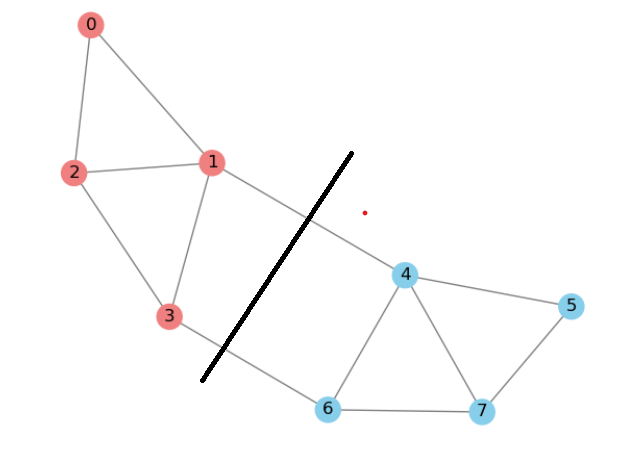
\includegraphics[width=0.9\linewidth]{Maths-Beamer-Overleaf/images/image06.png}
    \vspace{1mm}
    \textbf{Spectral Partitioned Graph}
\end{column}

% Right Column: Matrices and Values
\begin{column}{0.48\textwidth}
    \scriptsize
    \textbf{Laplacian Matrix:}
    
    \vspace{1mm}
    \adjustbox{max width=\linewidth}{
    \[
    \begin{bmatrix}
    2 & -1 & 0 & -1 & 0 & 0 & 0 & 0 \\
    -1 & 4 & -1 & -1 & -1 & 0 & 0 & 0 \\
    0 & -1 & 3 & -1 & 0 & 0 & 0 & -1 \\
    -1 & -1 & -1 & 3 & 0 & 0 & 0 & 0 \\
    0 & -1 & 0 & 0 & 4 & -1 & -1 & -1 \\
    0 & 0 & 0 & 0 & -1 & 2 & -1 & 0 \\
    0 & 0 & 0 & 0 & -1 & -1 & 3 & -1 \\
    0 & 0 & -1 & 0 & -1 & 0 & -1 & 3 \\
    \end{bmatrix}
    \]
    }

    \vspace{2mm}
    \textbf{Fiedler Vector:}
    
    \vspace{1mm}
    \adjustbox{max width=\linewidth}{
    \(
    \begin{bmatrix}
    0.4886, 0.2503, 0.1953, 0.4006, -0.2503, -0.4886, -0.4006, -0.1953 
    \end{bmatrix}
    \)
    }

    \vspace{2mm}
    \textbf{Lost Edges between \(G_1\) and \(G_2\): 2}

\end{column}
\end{columns}
\end{frame}

\begin{frame}
\textbf{Example 02}
\begin{columns}

% Left Column: Graph Image
\begin{column}{0.45\textwidth}
    \centering
    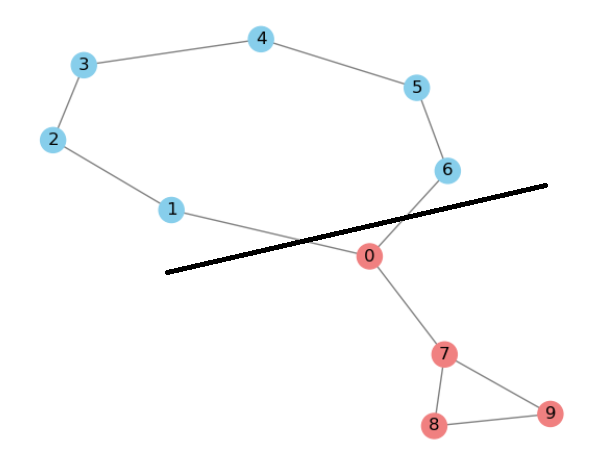
\includegraphics[width=0.9\linewidth]{Maths-Beamer-Overleaf/images/image05.png}
    \vspace{1mm}
    \textbf{Spectral Partitioned Graph}
\end{column}

% Right Column: Matrices and Values
\begin{column}{0.48\textwidth}
    \scriptsize
    \textbf{Laplacian Matrix:}
    
    \vspace{1mm}
    \adjustbox{max width=\linewidth}{
    \[
    \begin{bmatrix}
     3 & -1 & 0 & 0 & 0 & 0 & -1 & -1 & 0 & 0 \\
    -1 & 2 & -1 & 0 & 0 & 0 & 0  & 0  & 0 & 0 \\
     0 & -1 & 2 & -1 & 0 & 0 & 0  & 0  & 0 & 0 \\
     0 &  0 & -1 & 2 & -1 & 0 & 0  & 0  & 0 & 0 \\
     0 &  0 & 0 & -1 & 2 & -1 & 0  & 0  & 0 & 0 \\
     0 &  0 & 0 & 0  & -1 & 2 & -1 & 0  & 0 & 0 \\
    -1 &  0 & 0 & 0  & 0  & -1 & 2  & 0  & 0 & 0 \\
    -1 &  0 & 0 & 0  & 0  & 0  & 0  & 3  & -1 & -1 \\
     0 &  0 & 0 & 0  & 0  & 0  & 0  & -1 & 2  & -1 \\
     0 &  0 & 0 & 0  & 0  & 0  & 0  & -1 & -1 & 2 \\
    \end{bmatrix}
    \]
    }

    \vspace{2mm}
    \textbf{Fiedler Vector:}
    
    \vspace{1mm}
    \adjustbox{max width=\linewidth}{
    \(
    \begin{bmatrix}
    0.0521, -0.1147, -0.2543, -0.3335, -0.3335, -0.2543, -0.1147, 0.3734, 0.4897, 0.4897
    \end{bmatrix}
    \)}

    \vspace{2mm}
    \textbf{Lost Edges between \(G_1\) and \(G_2\): 2}

\end{column}
\end{columns}
\end{frame}

\begin{frame}{Industrial Applications}
    \begin{itemize}
        \item \textbf{Community Detection:} Identify clusters in social or information networks.
        \item \textbf{Image Segmentation:} Partition images into regions based on similarity.
        \item \textbf{Web Graph Analysis:} Analyze internet topology or hyperlink networks.
        \item \textbf{Biological Networks:} Discover functional modules in gene or protein networks.
        \item \textbf{VLSI Design:} Efficiently partition circuits for chip design.
        \item \textbf{Parallel Computing:} Divide tasks while minimizing inter-process communication.
    \end{itemize}
\end{frame}

\begin{frame}{Limitations of Spectral Partitioning}

\begin{columns}

    % Left column with text
    \begin{column}{0.7\textwidth}
        \textbf{Although Fiedler's Spectral Partitioning works well in many cases, it has limitations:}

        \vspace{0.3cm}
        \textbf{Examples of cases where it struggles:}
        \begin{itemize}
            \item \textbf{Star Graph:} A graph with one central vertex connected to all others \textbf{(as shown in figure)}.\\ Since, removing central edge removes all edges and graaph becomes disconnected
            \item Graphs with highly skewed degree distributions.
            \item Graphs where edge density is unevenly concentrated.
        \end{itemize}

        \vspace{0.3cm}
        \textbf{Why it fails:} In these cases, the second smallest eigenvalue (Fiedler value) and the corresponding eigenvector may not produce a balanced or meaningful partition.

    \end{column}

    % Right column with image
    \begin{column}{0.3\textwidth}
        \begin{figure}
            \centering
            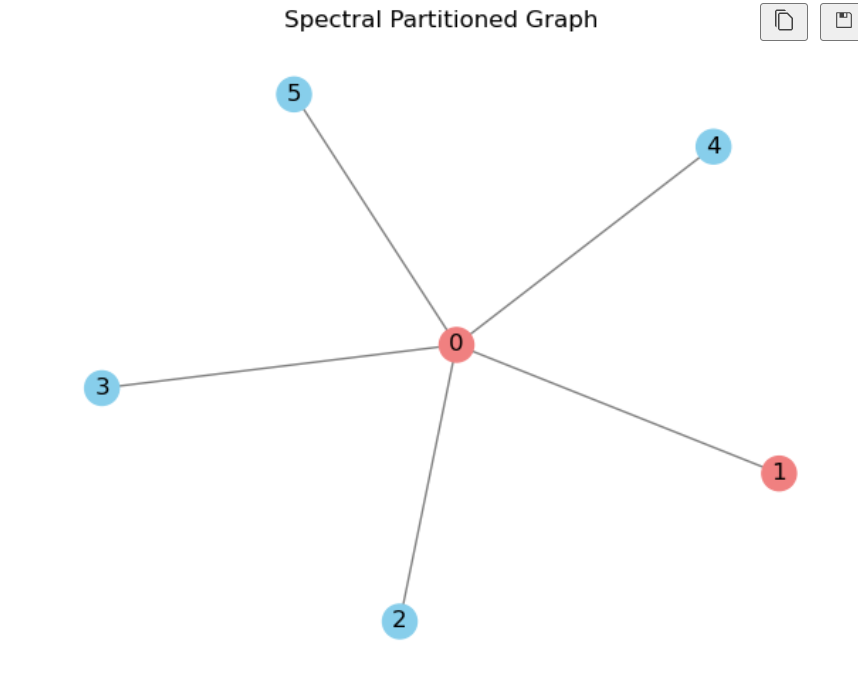
\includegraphics[width=.9\textwidth]{Maths-Beamer-Overleaf/images/image09.png}
            \caption*{\small Star Graph Example}
        \end{figure}
    \end{column}

\end{columns}

\end{frame}



\begin{frame}{Further Work after Fiedler's Decomposition}
\begin{itemize}
    \item \textbf{Multiway Spectral Clustering:} Use multiple eigenvectors (beyond the second smallest) for \( k \)-way graph partitioning.
    \item \textbf{Graph Coarsening:} Combine with graph reduction techniques (like collapsing and merging) to simplify large graphs for efficient computations.
    \item \textbf{Dynamic Graphs:} Combine other methods like anomaly detection and then apply Fiedler decomposition.
    \item \textbf{Spectral Embedding:} Use multiple eigenvectors to embed graphs in 2D/3D for visualization and pattern discovery.
    \item \textbf{Graph Signal Processing:} Treat Fiedler vector as a low-frequency graph signal for tasks like denoising and filtering.
\end{itemize}
\end{frame}


\begin{frame}{Conclusion}
    \begin{itemize}
        \item We explored the theory and application of \textbf{Spectral Graph Partitioning} using the \textbf{Fiedler vector}.
        \item The graph Laplacian \( L(G) \) was constructed from the adjacency and degree matrices of each graph.
        \item The \textbf{second smallest eigenvector} of the Laplacian, known as the Fiedler vector, was used to divide the graph into two meaningful partitions.
        \item Example graphs demonstrated that this approach is both interpretable and effective in detecting natural partitions.
        \item Visualizations of graphs and their matrix forms validated the partitioning process.
    \end{itemize}
\end{frame}



\begin{frame}{References}
    \begin{itemize}
        \item \href{https://www.youtube.com/watch?v=siCPjpUtE0A&t=1s}{Spectral Graph Partitioning – Finding a Partition (YouTube)}
        \item James Demmel. \textit{Graph Partitioning, Part 1}. Available at: \\
        \url{http://www.cs.berkeley.edu/~demmel/cs267/lecture18/lecture18.html} (1996)
        \item James Demmel. \textit{Graph Partitioning, Part 2}. Available at: \\
        \url{http://www.cs.berkeley.edu/~demmel/cs267/lecture20/lecture20.html} (1999)
        \item Basic Graph Theory - GeeksForGeeks: \\
        \url{https://www.geeksforgeeks.org/fundamentals-of-graph-theory/}
        \item \textbf{All resources are available at: \url{https://github.com/AyushmanGHub/Fiedlers-Spectral-Graph-Partitioning-Paper/}}
    \end{itemize}
\end{frame}

\end{document}
